\section{Data to Monte Carlo comparisons at $\sqrt{s}=2.36$ TeV in
  Minimum Bias events}


\subsection{Basic $\etmiss$-related distributions.}
$\etmiss$ plots, Sumet plots, in EB/EE etc.

\subsection{$\etmiss$ resolution.}

\begin{figure}[h!]
 \centering
 \begin{tabular}{ll}
  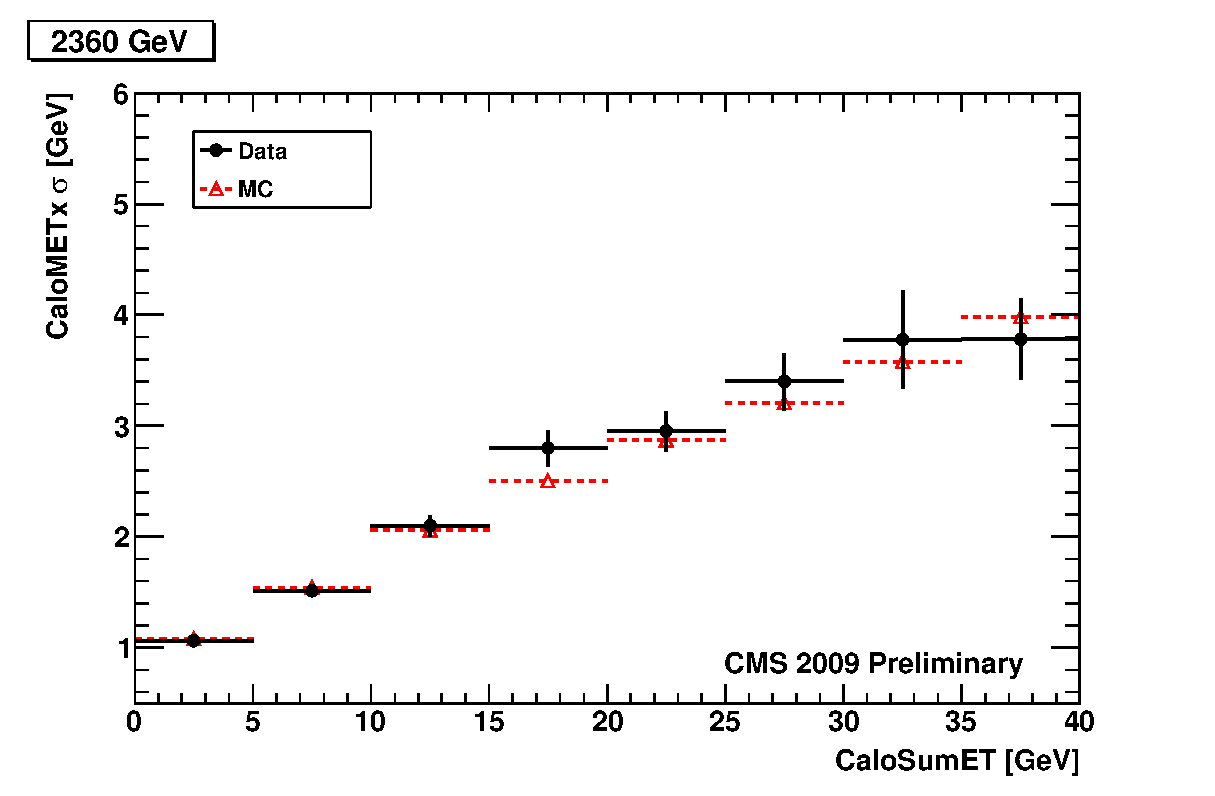
\includegraphics[width=0.5\textwidth]{plots_DataVsMC_MB_2360GeV/h_metxsigma_sumet_2360.eps} &
  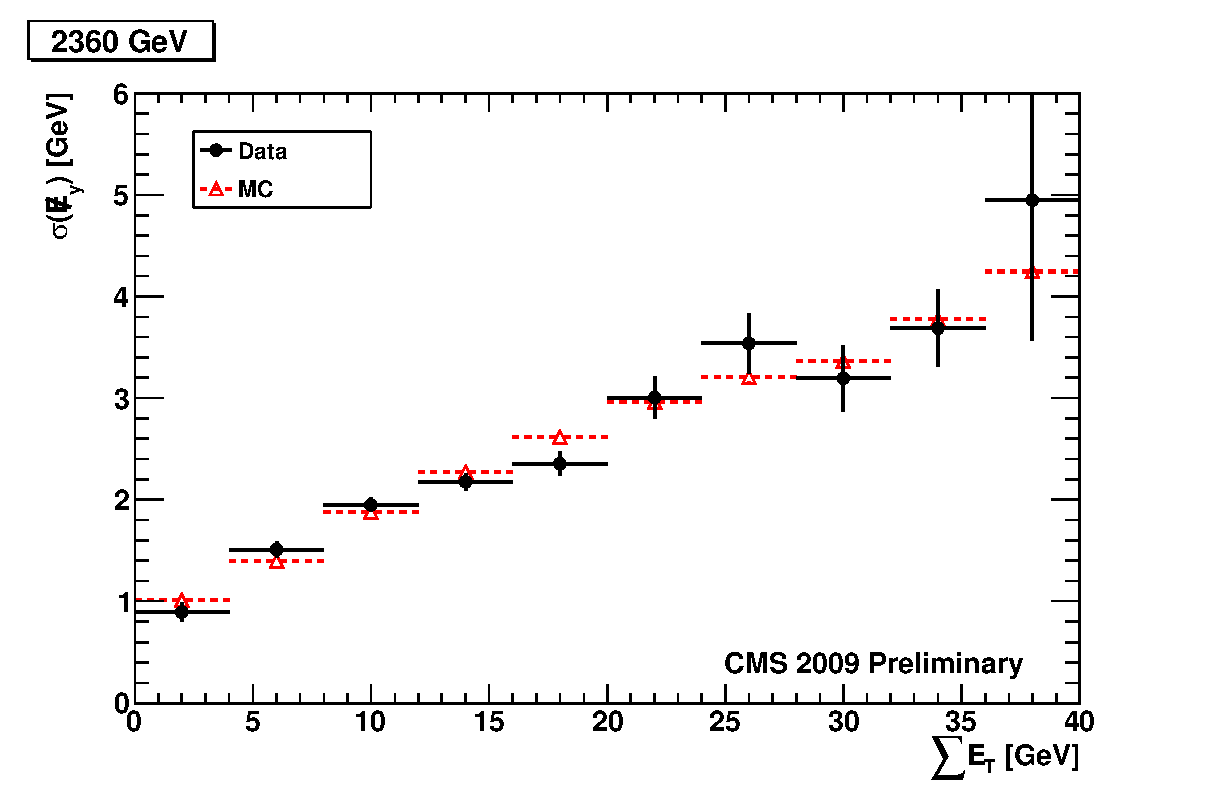
\includegraphics[width=0.5\textwidth]{plots_DataVsMC_MB_2360GeV/h_metysigma_sumet_2360.eps} \\
 \end{tabular}
 \caption{\small Comparison of the $\exmiss$ $\sigma$ vs. $\sum E_\text{T}$ and $\eymiss$ $\sigma$ vs. $\sum E_\text{T}$ between 
          Monte Carlo and data at $2360$ GeV.\label{fig:MExySigma_vs_SumET_2360}}
\end{figure}

\begin{figure}[h!]
 \centering
 \begin{tabular}{ll}
  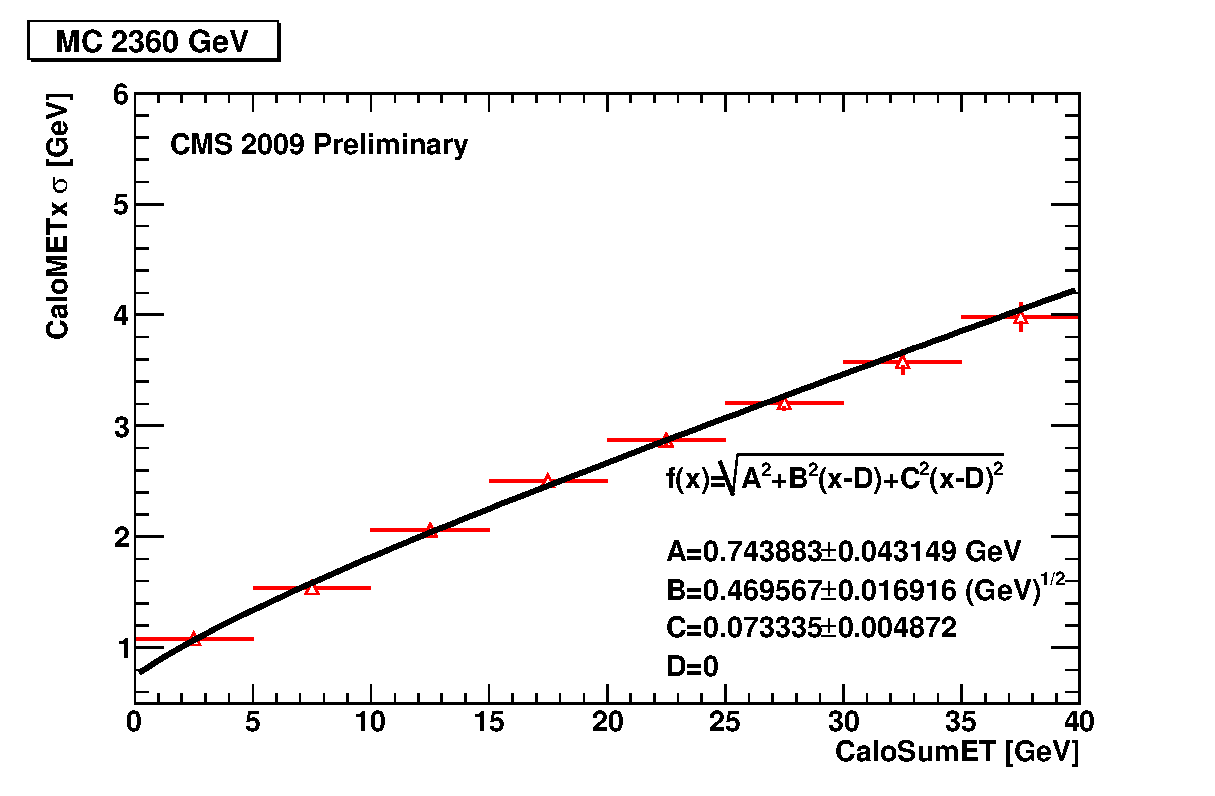
\includegraphics[width=0.5\textwidth]{plots_DataVsMC_MB_2360GeV/final_metxsigma_sumet_MC_2360.eps} &
  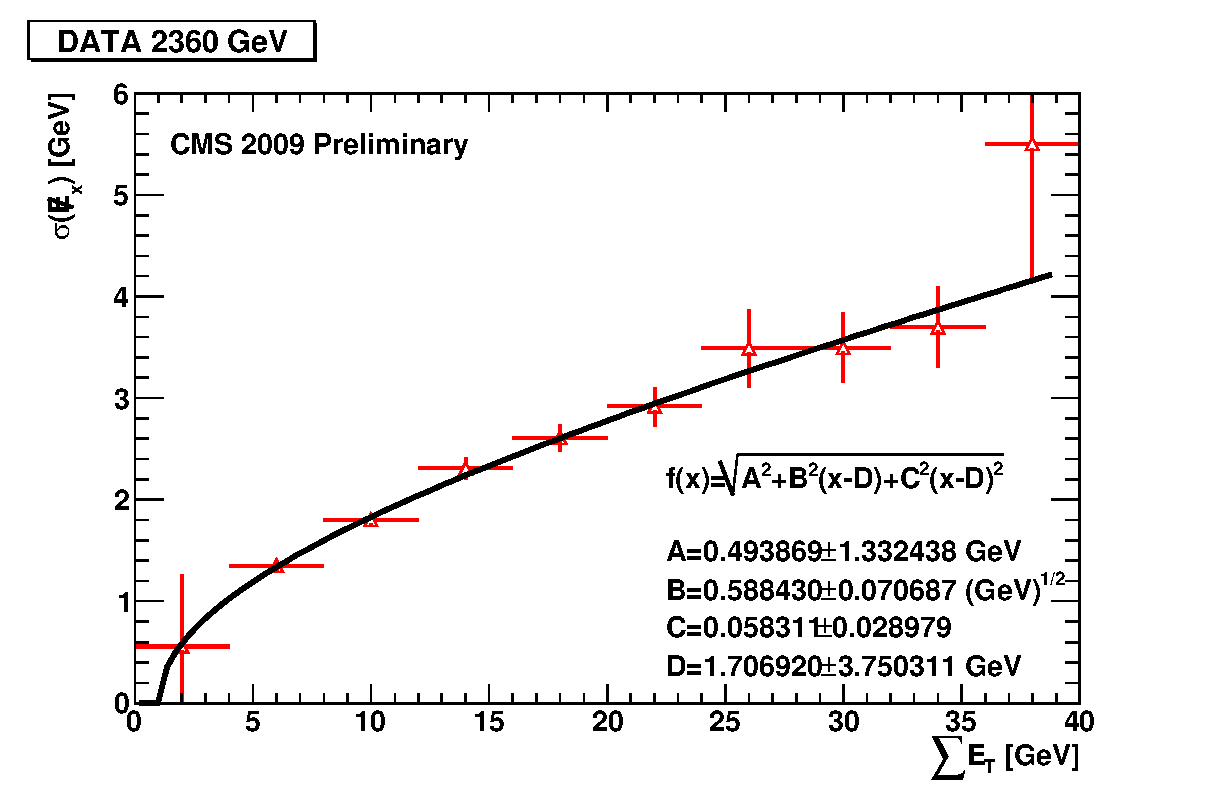
\includegraphics[width=0.5\textwidth]{plots_DataVsMC_MB_2360GeV/final_metxsigma_sumet_DATA_2360.eps} \\
 \end{tabular}
 \caption{\small Fit of the $\exmiss$ $\sigma$ vs. $\sum E_\text{T}$ for Monte Carlo and data at $2360$ GeV. Parameter $D$ in the fit was fixed
          to zero.\label{fig:MExSigma_vs_SumET_2360_fit}}
\end{figure}

\begin{figure}[h!]
 \centering
 \begin{tabular}{ll}
  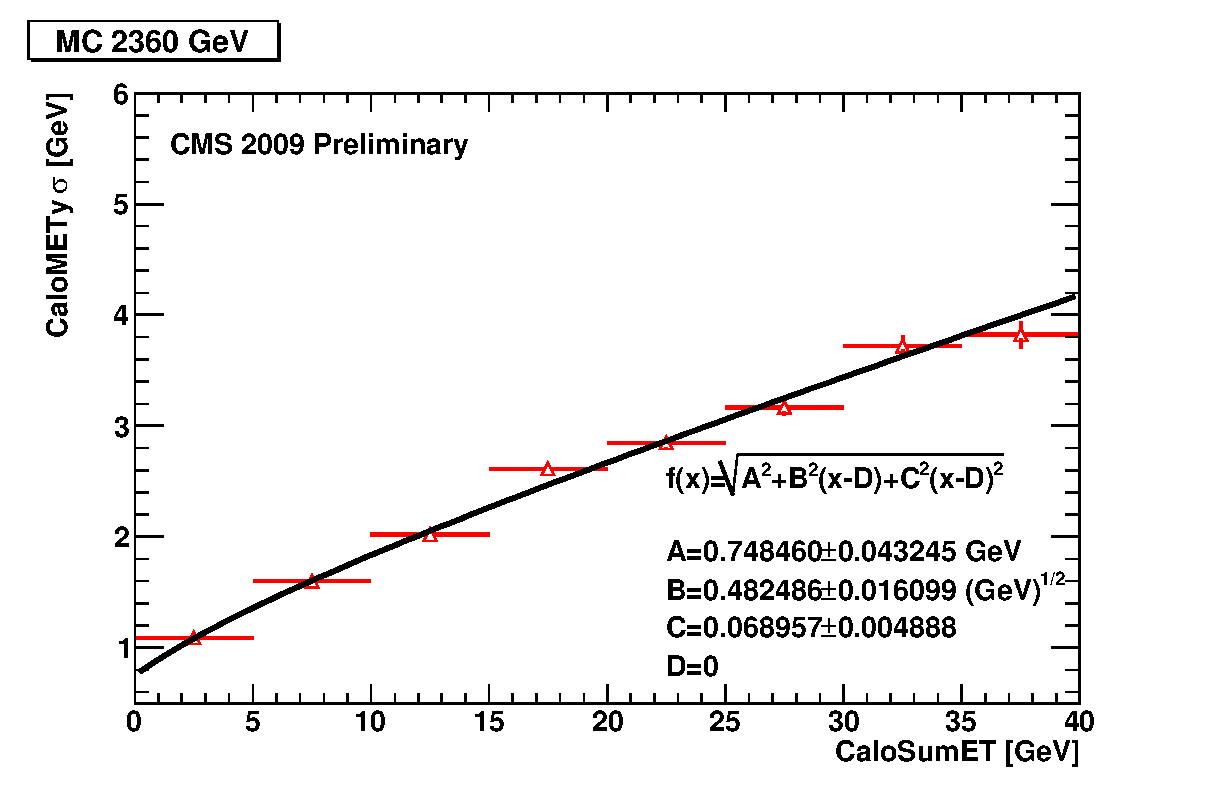
\includegraphics[width=0.5\textwidth]{plots_DataVsMC_MB_2360GeV/final_metysigma_sumet_MC_2360.eps} &
  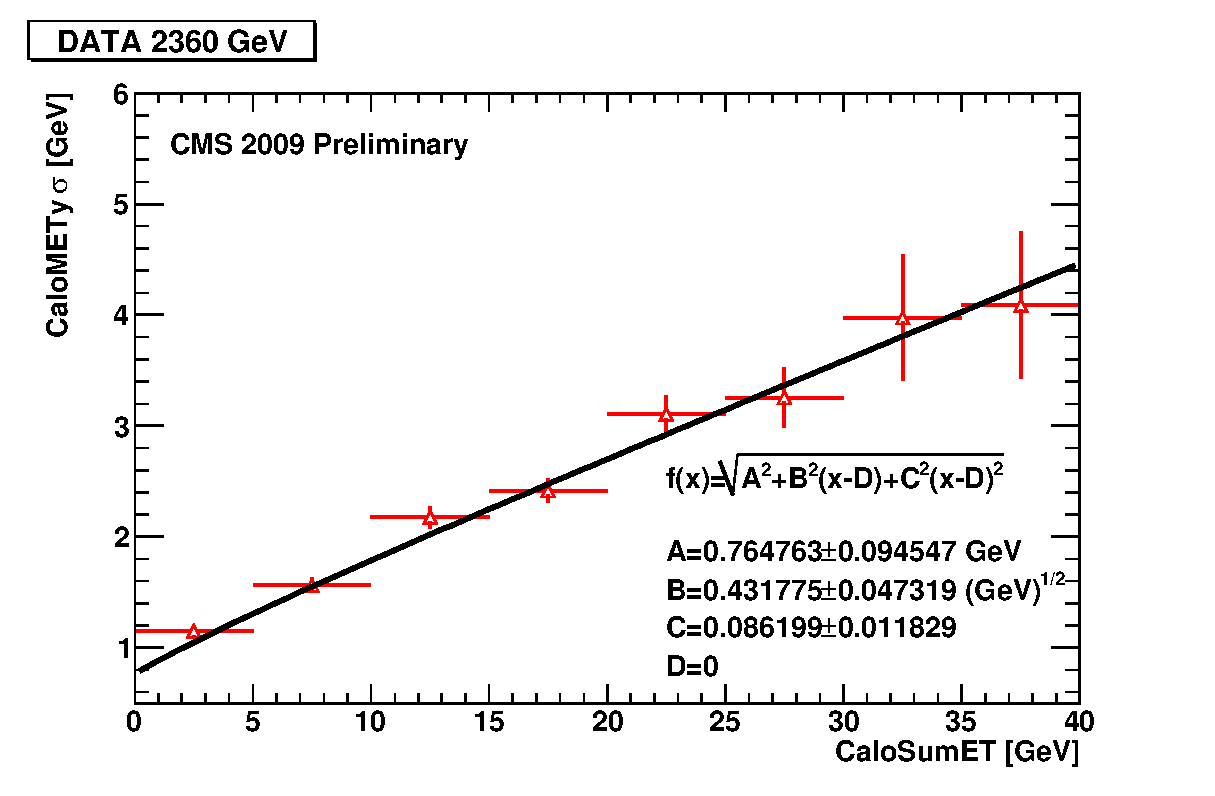
\includegraphics[width=0.5\textwidth]{plots_DataVsMC_MB_2360GeV/final_metysigma_sumet_DATA_2360.eps} \\
 \end{tabular}
 \caption{\small Fit of the $\eymiss$ $\sigma$ vs. $\sum E_\text{T}$ for Monte Carlo and data at $2360$ GeV. Parameter $D$ in the fit was fixed
          to zero.\label{fig:MExSigma_vs_SumET_2360_fit}}
\end{figure}

\subsection{$\etmiss$ and SumET dependence on $\eta$}
put here plots of MET VS etaring

